This section describes the typical persona, who is going to use this product. This document helps to identify the target user groups for the client version.
\begin{itemize}
    \item \textbf{End Users}: The general user cares about stuffs in cities. It is important for these users that the public infrastructures are working correctly to prevent dirty places, accidents and to make places more attractive. The end users are willing to use a mobile device to report detected issues and maybe become happy to receive a small gift for their reporting efforts.
    
    \begin{figure}[h]
        \centering
        \caption{User uses the application}
        \label{fig:user-uses-the-app}
        \begin{minipage}{0.4\textwidth}
            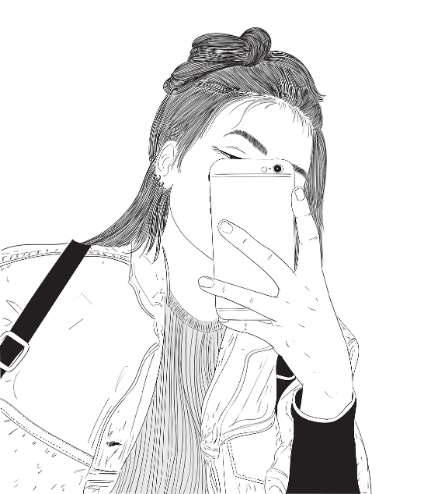
\includegraphics[width=\linewidth]{images/Image_ (1).png} 
        \end{minipage}%
        \hspace{0.05\textwidth} % Space between the image and the text
        \begin{minipage}{0.5\textwidth}
            I like to use my smartphone to take a picture and report this issue!
            \begin{enumerate}
                \item Just open the app.
                \item Make a new report.
                \item Select a category.
                \item Add multimedia (i.e., picture, video, voice).
                \item Add address or use geo location information.
                \item Press on submit button.
                \item You will be updated regarding the progress.
            \end{enumerate}
        \end{minipage}
    \end{figure}
    
    \item \textbf{Officer Users}: These users are officers in the authorities. As an officer user, they want to have a nice overview of all the reported issues, so that they can easily prepare the process of fixing those issues. They would like to export the reports data to some other application or send some emails to someone by those attached data or even maybe they have the possibility to make a workflow for resolving process in some other applications like SAP!

\end{itemize}

